
\documentclass[a4paper,10pt]{article}

\usepackage[utf8x]{inputenc}
\usepackage[textwidth=170mm,textheight=229mm]{geometry}
\usepackage{graphicx}
\usepackage{amsmath}
\usepackage{fancybox}
\usepackage{cancel}
\usepackage{wrapfig}
\usepackage{amsmath,amssymb,amsfonts,mathrsfs}
\usepackage{color}
\usepackage{slashed}
\usepackage{bbm}  
\usepackage{xspace}
\usepackage{subcaption}
\usepackage{multicol}
\usepackage{tikz}
\usetikzlibrary{arrows,shapes}
\usetikzlibrary{trees}
\usetikzlibrary{matrix,arrows} 				% For commutative diagram
											% http://www.felixl.de/commu.pdf
\usetikzlibrary{positioning}				% For "above of=" commands
\usetikzlibrary{calc,through}				% For coordinates
\usetikzlibrary{decorations.pathreplacing}  % For curly braces
% http://www.math.ucla.edu/~getreuer/tikz.html
\usepackage{pgffor}							% For repeating patterns

\usetikzlibrary{decorations.pathmorphing}	% For Feynman Diagrams
\usetikzlibrary{decorations.markings}
\tikzset{
	% >=stealth', %%  Uncomment for more conventional arrows
    vector/.style={decorate, decoration={snake}, draw},
	provector/.style={decorate, decoration={snake,amplitude=2.5pt}, draw},
	antivector/.style={decorate, decoration={snake,amplitude=-2.5pt}, draw},
    fermion/.style={draw=black, postaction={decorate},
        decoration={markings,mark=at position .55 with {\arrow[draw=black]{>}}}},
    fermionbar/.style={draw=black, postaction={decorate},
        decoration={markings,mark=at position .55 with {\arrow[draw=black]{<}}}},
    fermionnoarrow/.style={draw=black},
    gluon/.style={decorate, draw=black,
        decoration={coil,amplitude=4pt, segment length=5pt}},
    scalar/.style={dashed,draw=black, postaction={decorate},
        decoration={markings,mark=at position .55 with {\arrow[draw=black]{>}}}},
    scalarbar/.style={dashed,draw=black, postaction={decorate},
        decoration={markings,mark=at position .55 with {\arrow[draw=black]{<}}}},
    scalarnoarrow/.style={dashed,draw=black},
    electron/.style={draw=black, postaction={decorate},
        decoration={markings,mark=at position .55 with {\arrow[draw=black]{>}}}},
	bigvector/.style={decorate, decoration={snake,amplitude=4pt}, draw},
}\usetikzlibrary{decorations.markings}

% TIKZ - for block diagrams, 
% from http://www.texample.net/tikz/examples/control-system-principles/
% \usetikzlibrary{shapes,arrows}
\tikzstyle{block} = [draw, rectangle, 
    minimum height=3em, minimum width=6em]

%Definiciones
\newcommand{\phidag}{\phi^{\dagger}}
\newcommand{\vdag[1]}{V^{\dagger}_{#1}}
\newcommand{\Vdag[1]}{V^{#1\dagger}}
\newcommand{\Lbar}{\overline{L}}
\newcommand{\PL}{\frac{(1+\gamma_5)}{2}}
\newcommand{\PR}{\frac{(1-\gamma_5)}{2}}
\newcommand{\ld[1]}{\lambda_{#1}}
\newcommand{\Mv[1]}{M_{V_{#1}}}
\newcommand{\Mvc}{M_{V^{\pm}}}

\title{\textbf{Dark Vector Doublet Model (DVDM)}}
\begin{document}
\maketitle
%\tableofcontents

\section{Signatures from DVDM at the LHC} 
Due to the great similarity of the DVDM with respect to the i2HDM it is posible to reproduce the same mono-jet signature at LHC. The feynamn diagrams that contribute to the mono-jet signature are $gg\to V_1 V_1+$jet, $gq\to V_1 V_1+$jet and $q\overline{q}\to V_1 V_1+$jet which are presented in Fig(\ref{fig:fd-monojet1})
\begin{figure}[ht]
\centering
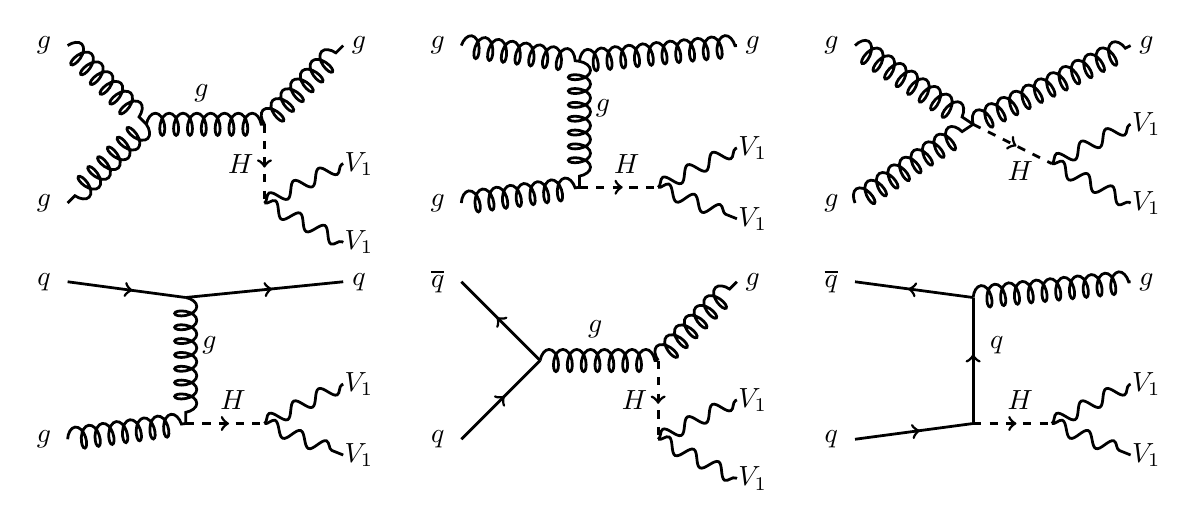
\begin{tikzpicture}[line width=1.0 pt, scale=1]
\begin{scope}[shift={(0,0)}]
	\draw[gluon](-1,1) -- (0,0);
	\draw[gluon](0,0) -- (-1,-1);
	\draw[gluon](0,0) -- (1.5,0);
	\draw[gluon](1.5,0) -- (2.5,1);
	\draw[scalar](1.5,0) -- (1.5,-1);
	\draw[vector](1.5,-1) -- (2.5, -0.5);
	\draw[vector](1.5,-1) -- (2.5, -1.5);
	\node at (-1.3,1) {$g$};
	\node at (-1.3,-1) {$g$};
	\node at (0.7,0.4) {$g$};
	\node at (2.7,1) {$g$};
	\node at (1.2,-0.5) {$H$};
	\node at (2.7,-0.5) {$V_1$};
	\node at (2.7,-1.5) {$V_1$};
\end{scope}
\begin{scope}[shift={(5,0)}]
	\draw[gluon](-1,1) -- (0.5,0.8);
	\draw[gluon](-1,-1) -- (0.5,-0.8);
	\draw[gluon](0.5,0.8) -- (0.5,-0.8);
	\draw[gluon](0.5,0.8) -- (2.5,1);
	\draw[scalar](0.5,-0.8) -- (1.5,-0.8);
	\draw[vector](1.5,-0.8) -- (2.5, -0.3);
	\draw[vector](1.5,-0.8) -- (2.5, -1.2);
	\node at (-1.3,1) {$g$};
	\node at (-1.3,-1) {$g$};
	\node at (0.8,0.2) {$g$};
	\node at (2.7,1) {$g$};
	\node at (1.1,-0.5) {$H$};
	\node at (2.7,-0.3) {$V_1$};
	\node at (2.7,-1.2) {$V_1$};
\end{scope}
\begin{scope}[shift={(10,0)}]
	\draw[gluon](-1,1) -- (0.5,0);
	\draw[gluon](-1,-1) -- (0.5,0);
	\draw[gluon](0.5,0) -- (2.5,1);
	\draw[scalar](0.5,0) -- (1.5,-0.5);
	\draw[vector](1.5,-0.5) -- (2.5, 0);
	\draw[vector](1.5,-0.5) -- (2.5, -1);
	\node at (-1.3,1) {$g$};
	\node at (-1.3,-1) {$g$};
	\node at (2.7,1) {$g$};
	\node at (1.1,-0.6) {$H$};
	\node at (2.7,0) {$V_1$};
	\node at (2.7,-1) {$V_1$};
\end{scope}
\begin{scope}[shift={(0,-3)}]
	\draw[fermion](-1,1) -- (0.5,0.8);
	\draw[gluon](-1,-1) -- (0.5,-0.8);
	\draw[gluon](0.5,0.8) -- (0.5,-0.8);
	\draw[fermion](0.5,0.8) -- (2.5,1);
	\draw[scalar](0.5,-0.8) -- (1.5,-0.8);
	\draw[vector](1.5,-0.8) -- (2.5, -0.3);
	\draw[vector](1.5,-0.8) -- (2.5, -1.2);
	\node at (-1.3,1) {$q$};
	\node at (-1.3,-1) {$g$};
	\node at (0.8,0.2) {$g$};
	\node at (2.7,1) {$q$};
	\node at (1.1,-0.5) {$H$};
	\node at (2.7,-0.3) {$V_1$};
	\node at (2.7,-1.2) {$V_1$};
\end{scope}
\begin{scope}[shift={(5,-3)}]
	\draw[fermion](0,0) -- (-1,1);
	\draw[fermion](-1,-1) -- (0,0);
	\draw[gluon](0,0) -- (1.5,0);
	\draw[gluon](1.5,0) -- (2.5,1);
	\draw[scalar](1.5,0) -- (1.5,-1);
	\draw[vector](1.5,-1) -- (2.5, -0.5);
	\draw[vector](1.5,-1) -- (2.5, -1.5);
	\node at (-1.3,1) {$\overline{q}$};
	\node at (-1.3,-1) {$q$};
	\node at (0.7,0.4) {$g$};
	\node at (2.7,1) {$g$};
	\node at (1.2,-0.5) {$H$};
	\node at (2.7,-0.5) {$V_1$};
	\node at (2.7,-1.5) {$V_1$};
\end{scope}
\begin{scope}[shift={(10,-3)}]
	\draw[fermion](0.5,0.8) -- (-1,1);
	\draw[fermion](-1,-1) -- (0.5,-0.8);
	\draw[fermion](0.5,-0.8) -- (0.5,0.8);
	\draw[gluon](0.5,0.8) -- (2.5,1);
	\draw[scalar](0.5,-0.8) -- (1.5,-0.8);
	\draw[vector](1.5,-0.8) -- (2.5, -0.3);
	\draw[vector](1.5,-0.8) -- (2.5, -1.2);
	\node at (-1.3,1) {$\overline{q}$};
	\node at (-1.3,-1) {$q$};
	\node at (0.8,0.2) {$q$};
	\node at (2.7,1) {$g$};
	\node at (1.1,-0.5) {$H$};
	\node at (2.7,-0.3) {$V_1$};
	\node at (2.7,-1.2) {$V_1$};
\end{scope}
\end{tikzpicture}
\caption{Feynman diagrams for $gg\to V_1 V_1+$jet, $gq\to V_1 V_1+$jet and $q\overline{q}\to V_1 V_1+$jet process contributing to mono-jet signature.} \label{fig:fd-monojet1}
\end{figure}
\newline
For this signature, the relevant non-trivial parameter space is two dimensional, in which the DM mass $\Mv[1]$ and the $\ld[L]$ parameter contribute to the cross section, however since the second parameter just scales the production cross section which is proportional to $\ld[L]^2$, we can consider the process like one dimensional parameter space.

\newpage
There is one more process which contributes to mono-jet signature from DVDM, namely $q\bar{q}\to V_1 V_2+g$ and $gq\to V_1 V_2+q$ process diagrams for which are presented in Fig.(\ref{fig:fd-monojet2}).
\begin{figure}[ht]
\centering
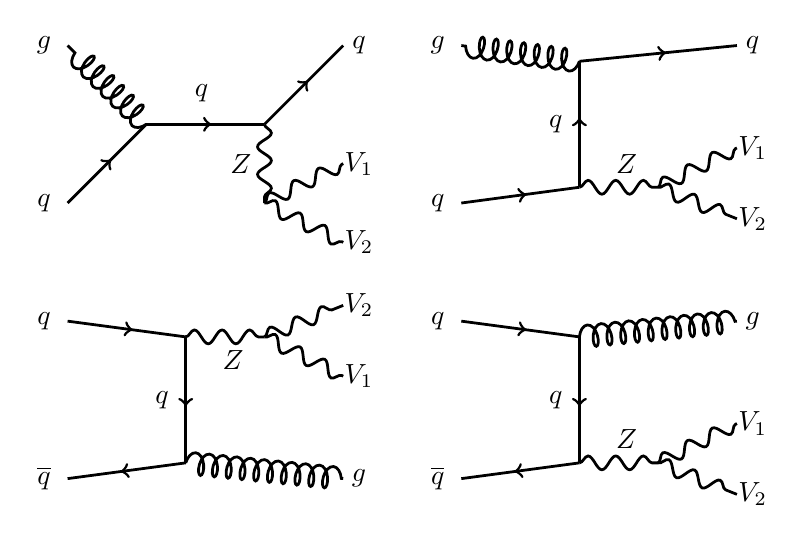
\begin{tikzpicture}[line width=1.0 pt, scale=1]
\begin{scope}[shift={(0,0)}]
	\draw[gluon](0,0) -- (-1,1);
	\draw[fermion](-1,-1) -- (0,0);
	\draw[fermion](0,0) -- (1.5,0);
	\draw[fermion](1.5,0) -- (2.5,1);
	\draw[vector](1.5,0) -- (1.5,-1);
	\draw[vector](1.5,-1) -- (2.5, -0.5);
	\draw[vector](1.5,-1) -- (2.5, -1.5);
	\node at (-1.3,1) {$g$};
	\node at (-1.3,-1) {$q$};
	\node at (0.7,0.4) {$q$};
	\node at (2.7,1) {$q$};
	\node at (1.2,-0.5) {$Z$};
	\node at (2.7,-0.5) {$V_1$};
	\node at (2.7,-1.5) {$V_2$};
\end{scope}
\begin{scope}[shift={(5,0)}]
	\draw[gluon](0.5,0.8) -- (-1,1);
	\draw[fermion](-1,-1) -- (0.5,-0.8);
	\draw[fermion](0.5,-0.8) -- (0.5,0.8);
	\draw[fermion](0.5,0.8) -- (2.5,1);
	\draw[vector](0.5,-0.8) -- (1.5,-0.8);
	\draw[vector](1.5,-0.8) -- (2.5, -0.3);
	\draw[vector](1.5,-0.8) -- (2.5, -1.2);
	\node at (-1.3,1) {$g$};
	\node at (-1.3,-1) {$q$};
	\node at (0.2,0) {$q$};
	\node at (2.7,1) {$q$};
	\node at (1.1,-0.5) {$Z$};
	\node at (2.7,-0.3) {$V_1$};
	\node at (2.7,-1.2) {$V_2$};
\end{scope}
\begin{scope}[shift={(0,-3.5)}]
	\draw[fermion](-1,1) -- (0.5,0.8);
	\draw[fermion](0.5,-0.8) -- (-1,-1);
	\draw[fermion](0.5,0.8) -- (0.5,-0.8);
	\draw[vector](0.5,0.8) -- (1.5,0.8);
	\draw[vector](1.5,0.8) -- (2.5, 0.3);
	\draw[vector](1.5,0.8) -- (2.5, 1.2);
	\draw[gluon](0.5,-0.8) -- (2.5,-1);
	\node at (-1.3,1) {$q$};
	\node at (-1.3,-1) {$\overline{q}$};
	\node at (0.2,0) {$q$};
	\node at (2.7,-1) {$g$};
	\node at (1.1,0.5) {$Z$};
	\node at (2.7,0.3) {$V_1$};
	\node at (2.7,1.2) {$V_2$};
\end{scope}
\begin{scope}[shift={(5,-3.5)}]
	\draw[fermion](-1,1) -- (0.5,0.8);
	\draw[fermion](0.5,-0.8) -- (-1,-1);
	\draw[fermion](0.5,0.8) -- (0.5,-0.8);
	\draw[gluon](0.5,0.8) -- (2.5,1);
	\draw[vector](0.5,-0.8) -- (1.5,-0.8);
	\draw[vector](1.5,-0.8) -- (2.5, -0.3);
	\draw[vector](1.5,-0.8) -- (2.5, -1.2);
	\node at (-1.3,1) {$q$};
	\node at (-1.3,-1) {$\overline{q}$};
	\node at (0.2,0) {$q$};
	\node at (2.7,1) {$g$};
	\node at (1.1,-0.5) {$Z$};
	\node at (2.7,-0.3) {$V_1$};
	\node at (2.7,-1.2) {$V_2$};
\end{scope}
\end{tikzpicture}
\caption{Feynman diagrams for $q\bar{q}\to V_1 V_2+g$ and $gq\to V_1 V_2+q$ process contributing to mono-jet signature.} \label{fig:fd-monojet2}
\end{figure}

%This process will contribute to the mono-jet signature in case of the small mass split between $h_1$ and $h_2$. In this case $h_2$ will decay to $h_1$ and soft jets and leptons, which cannot be detected. In spite of the fact that there is one  mediator for this process, the $Z$-boson, one can also see that $t-$ and $s-$channel topologies with the light quark in the propagator make this process different from simplified models with fermion dark matter and vector mediator which has been studied so far. For this mono-jet process the vertex $h_1h_2Z$ depends on the gauge constant, therefore the essential parameter space for this process is the two-dimensional $\Mh[1]-\Mh[2]$ plane which fixes its cross section. 
\begin{figure}[htb]
\centering
{\includegraphics[width=0.52\textwidth]{CM_limit_v1v1j_13TeV.pdf}}%
{\includegraphics[width=0.52\textwidth]{CM_limit_v1v2j_13TeV.pdf}}%
\vskip -0.5cm\hspace*{-3cm}(a)\hspace*{0.48\textwidth}(b)
\caption{Cross sections and 95\% CLs for $pp \to V_1 V_1 +$ jet versus $\Mv[1]$ at 13 TeV in figure a) and $pp \to V_1 V_2 +$ jet versus $\Mv[1]$ in figure b). In Fig a), the cross sections are shown for 3 different values of $\ld[L]$: (i) $\ld[L]=1$ ({\textbf{\color{blue} blue}} dashed), (ii) $\ld[L]= 5$ ({\textbf{\color{green} green}} dashed), (iii) $\ld[L]=10$  ({\textbf{\color{magenta} magenta}} dashed). In Fig b), the cross sections are shown for 3 different values of $\Delta M = \Mv[2] - \Mv[1]$: (i) $\Delta M=1$ GeV ({\textbf{\color{blue} blue}} dashed), (ii) $\Delta M= 10$ GeV ({\textbf{\color{green} green}} dashed), (iii) $\Delta M=100$ GeV ({\textbf{\color{magenta} magenta}} dashed). (a) Results for 13 TeV, with limits (solid {\textbf{\color{red} red}}) calculated using the ATLAS analysis from CheckMATE.}
\end{figure}

\newpage
\begin{figure}[htb]
\centering
{\includegraphics[width=0.52\textwidth]{Mv1_lamL_Omega_cut12345678.pdf}}%
{\includegraphics[width=0.52\textwidth]{Mv1_Mv2_Omega_cut12345678.pdf}}%
\vskip -0.5cm\hspace*{-3cm}(a)\hspace*{0.48\textwidth}(b)
\caption{Projection of the 5D random scan of the DVDM into the $(\Mv[1],\ld[L])$ plane and the excluded region at the LHC@13 TeV with 36.1 fb$^{-1}$ of integrated luminosity using $V_1 V_1 j$ channel}
\end{figure}

\begin{figure}[htb]
\centering
{\includegraphics[width=0.52\textwidth]{Mv1_lamL_Omega_cut12345679.pdf}}%
{\includegraphics[width=0.52\textwidth]{Mv1_Mv2_Omega_cut12345679.pdf}}%
\vskip -0.5cm\hspace*{-3cm}(a)\hspace*{0.48\textwidth}(b)
\caption{Projection of the 5D random scan of the DVDM into the $(\Mv[1],\ld[L])$ plane and the excluded region at the LHC@13 TeV with 36.1 fb$^{-1}$ of integrated luminosity using $V_1 V_2 j$ channel}
\end{figure}

\end{document}

